\documentclass{article}
\usepackage[utf8]{inputenc}
\usepackage{amsmath}
\usepackage{listings}
\usepackage{graphicx}

\graphicspath{{/home/pdro/Prog/introFISCOMP/2}}

\begin{document}
\section{Números aleatórios}

Criou-se um gerador congruente linear de números aleatórios sob a forma de uma subrotina, chamada GENRDM (de ``generate random number''). Seu funcionamento consistia em modificar uma variável inteira R, cujo valor inicial se nomeia ``semente'' ou ``seed'', para um novo valor randômico a cada chamada, segundo a seguinte expressão:


\begin{displaymath}
  \label{eq:gerador}
  R=MOD(aR+c, m)
\end{displaymath}

Em que MOD é a função nativa para a operação de módulo no FORTRAN e \(a\), \(c\) e \(m\) são parâmetros inteiros. \par
Para medir o período do gerador, armazenou-se a semente também em outra variável A1, e executou-se um laço DO WHILE (R /= A1), que chamava GENRDM em R e incrementava uma variável contadora a cada ciclo.\par
É importante notar que fez-se necessário chamar a subrotina uma única vez antes do laço, para impedir que o condicional R /= A1 fosse violado já na primeira execução do loop e este, portanto, nem iniciasse. Disso resulta que a contadora deve iniciar em 1.\par
O programa descrito, incrementado de impressões auxiliares, foi rodado a partir de cinco valores sementes distintos, com os parâmetros \(a=7\),\(c=4\) e \(m = 15\), culminando no seguinte output:

\begin{lstlisting}


 =====================================
 SEED:           1
 -------------------------------------
 R           1 :          11
 R           2 :           6
 -------------------------------------
 O PERIODO VALE           3
 =====================================
 SEED:           5
 -------------------------------------
 R           1 :           9
 R           2 :           7
 R           3 :           8
 R           4 :           0
 R           5 :           4
 R           6 :           2
 R           7 :           3
 R           8 :          10
 R           9 :          14
 R          10 :          12
 R          11 :          13
 -------------------------------------
 O PERIODO VALE          12
 =====================================
 SEED:          10
 -------------------------------------
 R           1 :          14
 R           2 :          12
 R           3 :          13
 R           4 :           5
 R           5 :           9
 R           6 :           7
 R           7 :           8
 R           8 :           0
 R           9 :           4
 R          10 :           2
 R          11 :           3
 -------------------------------------
 O PERIODO VALE          12
 =====================================
 SEED:           9
 -------------------------------------
 R           1 :           7
 R           2 :           8
 R           3 :           0
 R           4 :           4
 R           5 :           2
 R           6 :           3
 R           7 :          10
 R           8 :          14
 R           9 :          12
 R          10 :          13
 R          11 :           5
 -------------------------------------
 O PERIODO VALE          12
 =====================================
 SEED:          12
 -------------------------------------
 R           1 :          13
 R           2 :           5
 R           3 :           9
 R           4 :           7
 R           5 :           8
 R           6 :           0
 R           7 :           4
 R           8 :           2
 R           9 :           3
 R          10 :          10
 R          11 :          14
 -------------------------------------
 O PERIODO VALE          12



\end{lstlisting}

Percebe-se que, com exceção da seed 1, o período manteve-se o mesmo para qualquer valor inicial de R, só dependendo da escolha dos parâmetros.\par
Repetindo o processo para \(m = 17\), chega-se em:

\begin{lstlisting}


 =====================================
 SEED:           1
 -------------------------------------
 R           1 :          11
 R           2 :          13
 R           3 :          10
 R           4 :           6
 R           5 :          12
 R           6 :           3
 R           7 :           8
 R           8 :           9
 R           9 :          16
 R          10 :          14
 R          11 :           0
 R          12 :           4
 R          13 :          15
 R          14 :           7
 R          15 :           2
 -------------------------------------
 O PERIODO VALE          16
 =====================================
 SEED:           5
 -------------------------------------
 -------------------------------------
 O PERIODO VALE           1
 =====================================
 SEED:          10
 -------------------------------------
 R           1 :           6
 R           2 :          12
 R           3 :           3
 R           4 :           8
 R           5 :           9
 R           6 :          16
 R           7 :          14
 R           8 :           0
 R           9 :           4
 R          10 :          15
 R          11 :           7
 R          12 :           2
 R          13 :           1
 R          14 :          11
 R          15 :          13
 -------------------------------------
 O PERIODO VALE          16
 =====================================
 SEED:           9
 -------------------------------------
 R           1 :          16
 R           2 :          14
 R           3 :           0
 R           4 :           4
 R           5 :          15
 R           6 :           7
 R           7 :           2
 R           8 :           1
 R           9 :          11
 R          10 :          13
 R          11 :          10
 R          12 :           6
 R          13 :          12
 R          14 :           3
 R          15 :           8
 -------------------------------------
 O PERIODO VALE          16
 =====================================
 SEED:          12
 -------------------------------------
 R           1 :           3
 R           2 :           8
 R           3 :           9
 R           4 :          16
 R           5 :          14
 R           6 :           0
 R           7 :           4
 R           8 :          15
 R           9 :           7
 R          10 :           2
 R          11 :           1
 R          12 :          11
 R          13 :          13
 R          14 :          10
 R          15 :           6
 -------------------------------------
 O PERIODO VALE          16


\end{lstlisting}

Dessa vez, o caso da semente 5 mostrou-se sui generis. É perceptível que o laço não foi executado sequer uma vez, ou seja, R continua igual a A1 mesmo após GENRDM ser chamada, e a subrotina então forma uma sequência constante.

Em seguida, foi implementado o gerador "Padrão Mínimo" de Park e Miller adotando-se os parâmetros \(a = 7^5 = 16807\), \(c = 0\) e \(m = 2^{31}-1 = 2147483647\). Para evitar overflow de inteiros e o surgimento de números negativos inesperados, usou-se inteiros do tipo 2, que ocupam 8 bytes de memória. Para limitar os números gerados ao intervalo de 0 a 1, dividiu-se o resultado por m (somente ao imprimir, não modificando o valor de R).\par
Foram criadas cinco séries aleatórias de 100 termos, cada uma com uma seed diferente, e suas médias e desvio padrão foram determinados com um dos programas criados no último projeto:

\begin{lstlisting}


 =====================================================
 SEED = 1
 -----------------------------------------------------
 DESVIO PADRAO  0.293284121375065786568896829921955881      
 MED ARIT.      0.518424693383792600000000000000000180      
 MED GEOM.      0.348651828239896703535890463674271277      
 =====================================================
 SEED = 54321
 -----------------------------------------------------
 DESVIO PADRAO  0.283287161024228344284956382709503882      
 MED ARIT.      0.483871921197499999999999999999999892      
 MED GEOM.      0.363824768098287321453565857356002073      
 =====================================================
 SEED = 12345
 -----------------------------------------------------
 DESVIO PADRAO  0.292136756417067757435692622683129028      
 MED ARIT.      0.521857077044229999999999999999999742      
 MED GEOM.      0.368687452583532120042038121305474769      
 =====================================================
 SEED = 99999
 -----------------------------------------------------
 DESVIO PADRAO  0.256387595514920214994502526906606715      
 MED ARIT.      0.496924723992299999999999999999999900      
 MED GEOM.      0.379035744713097804485614577801251787      
 =====================================================
 SEED = 42
 -----------------------------------------------------
 DESVIO PADRAO  0.282532207080993034192227575690754296      
 MED ARIT.      0.461516261659699999999999999999999965      
 MED GEOM.      0.315404544483989380376142297185411374 


\end{lstlisting}
Todos os resultados distam por menos que 0.06 dos valores de convergência para conjuntos de dados estocásticos: 0.5 para a média aritmética, \(\frac{1}{2\sqrt{3}} = 0.288675...\) para o desvio padrão e \(\frac{1}{e}=0.367879...\) para a média geométrica.\par
Precisou-se fazer uso de reais de 16 bytes para permitir o cálculo da média geométrica em séries de até por volta de 800 termos, pois a operação de produto gerava números demasiadamente elevados para serem comportados nos tipos padrão, de 4 bytes.\par
As sequências geradas foram então plotadas em gráficos de dispersão:

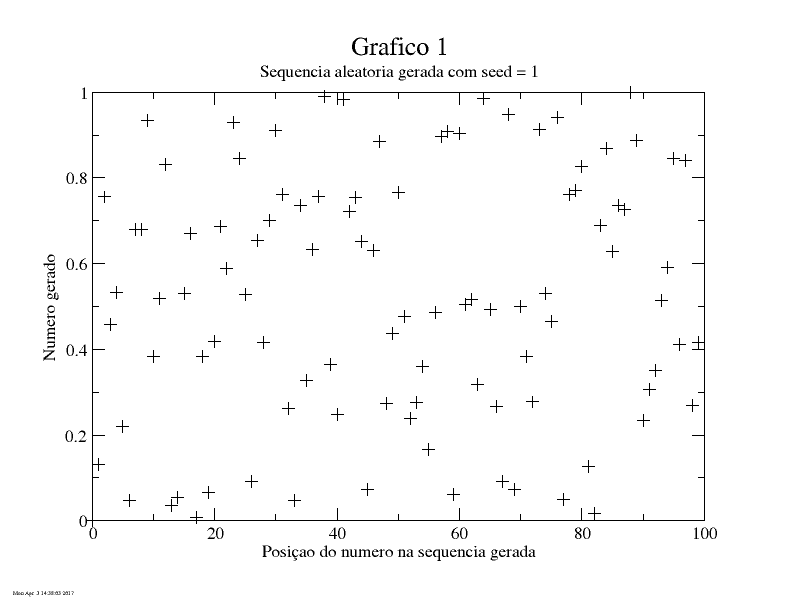
\includegraphics[width=\textwidth]{graf1}
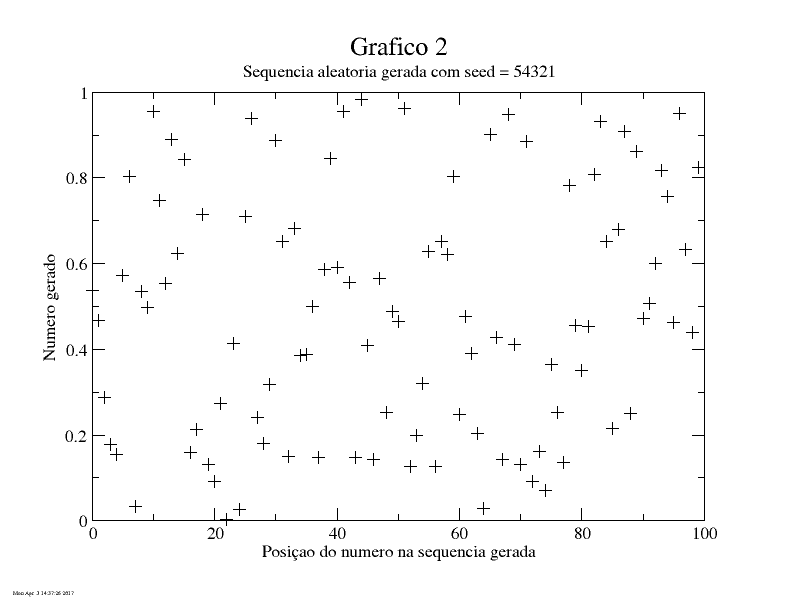
\includegraphics[width=\textwidth]{graf2}
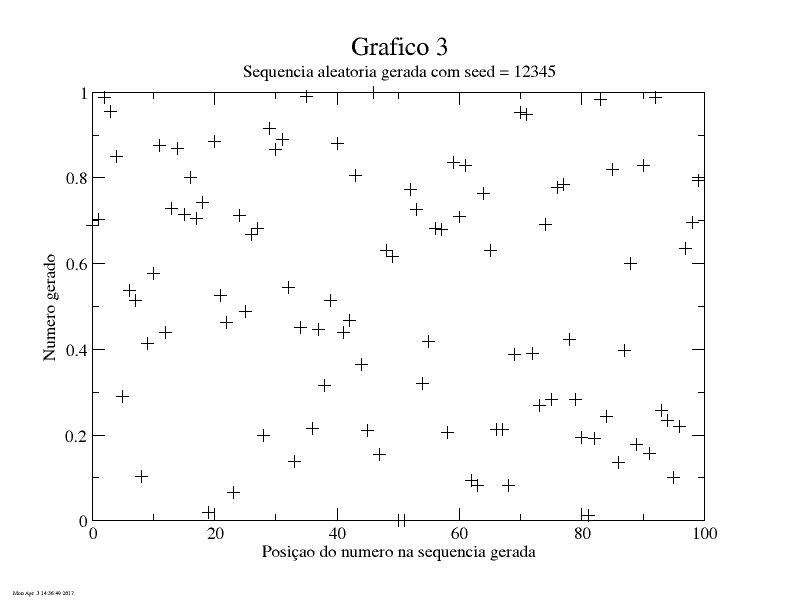
\includegraphics[width=\textwidth]{graf3}
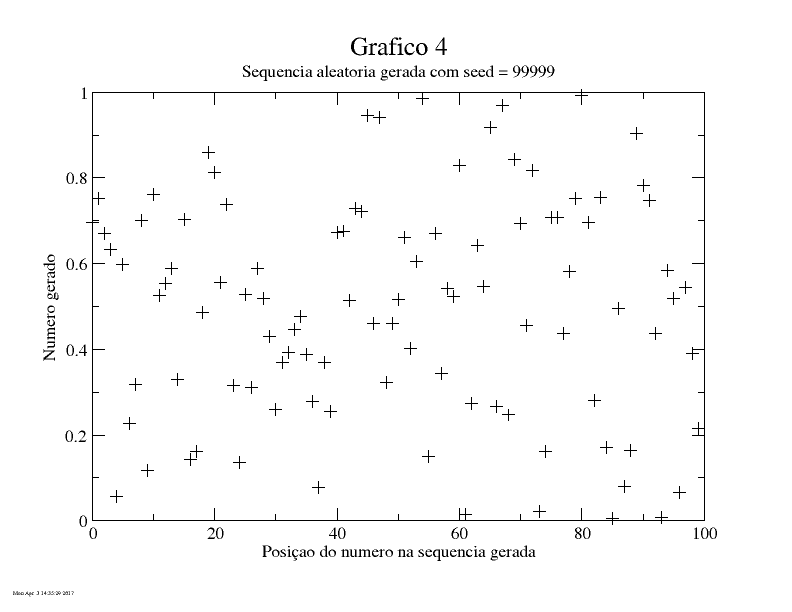
\includegraphics[width=\textwidth]{graf4}
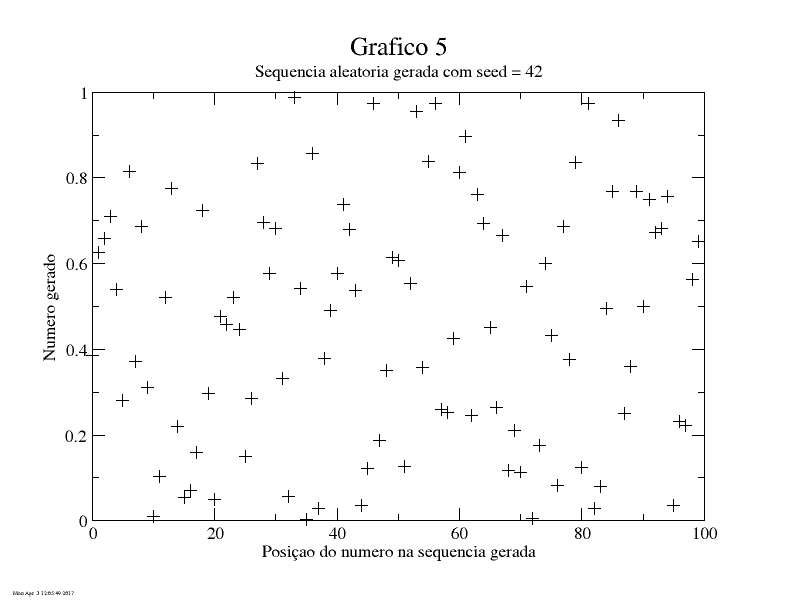
\includegraphics[width=\textwidth]{graf5}

Como esperado, a análise visual não revela nenhum padrão consistente nas representações gráficas. Tal desordem mostra-se útil em aplicações simples, menos formais, nas quais o rigor na aleatoriedade não se faz necessária.

\end{document}